\documentclass[12pt]{article}

\usepackage{graphicx}

\title{Report of FedWeb DesignLab Challenge}
\author{
        Han van der Veen \\ s1007130
            \and
			Rik van Outersterp \\ s1010875
}
\date{\today}

\begin{document}
\maketitle

%\begin{abstract}
%Aangezien het een verslag is en geen paper lijkt mij een abstract niet nodig.
%\end{abstract}

\section{Introduction}
This document elaborates our submission for the \textit{Design Challenge} assignment of the course \textit{Information Retrieval} at the University of Twente. 
For this assignment a web result page for aggregated web search had to designed.
The results of this web search consist of the results of multiple (independent) search engines.
The designed result page is planned to be used by the course' supervisors in a successive user experiment of which the purpose is to determine which pages give the best overall user experience, followed by a presentation of this study at the Text Retrieval Conference (TREC) in November 2014.

In this document we elaborate our web result pages.
The remainder of the document is setup as follows.
In section~\ref{sec:designs} our two designs are presented.
A proposal for evaluating our designs is presented in section~\ref{sec:evaluation}.
This document is concluded in section~\ref{sec:conclusion}.

\section{Designs}
\label{sec:designs}
Both our designs are build upon the same system.
The ranking of the search results is in both designs based on the title of the result.
A higher rank is achieved by a search result when the title contains the search term.
An even higher rank can be achieved when the title starts with the search term or even matches the search term exactly (note: case insensitive).

Since the assignment requires to have as many designs as group members, we have developed two designs.
We decided to put our own personal ideas in a design, such that two different designs were developed instead of two possibly very similar designs.
In the following subsections both designs are presented.

% Han's layout
\subsection{Design One}
\label{sec:layoutHan}
For the first design (Design One, see figure~\ref{fig:designOne}) we have chosen to blend in all the search engines.
By blending it together, all the results get the same amount of space in the layout and should be therefore considered as equally important. 
This allows the user to be able to determine the best result by himself instead of letting the system decide what the best result should be.
As mentioned this design uses the sorting system that was described in the beginning of section~\ref{sec:designs}.

\begin{figure}[h!]
  \centering
    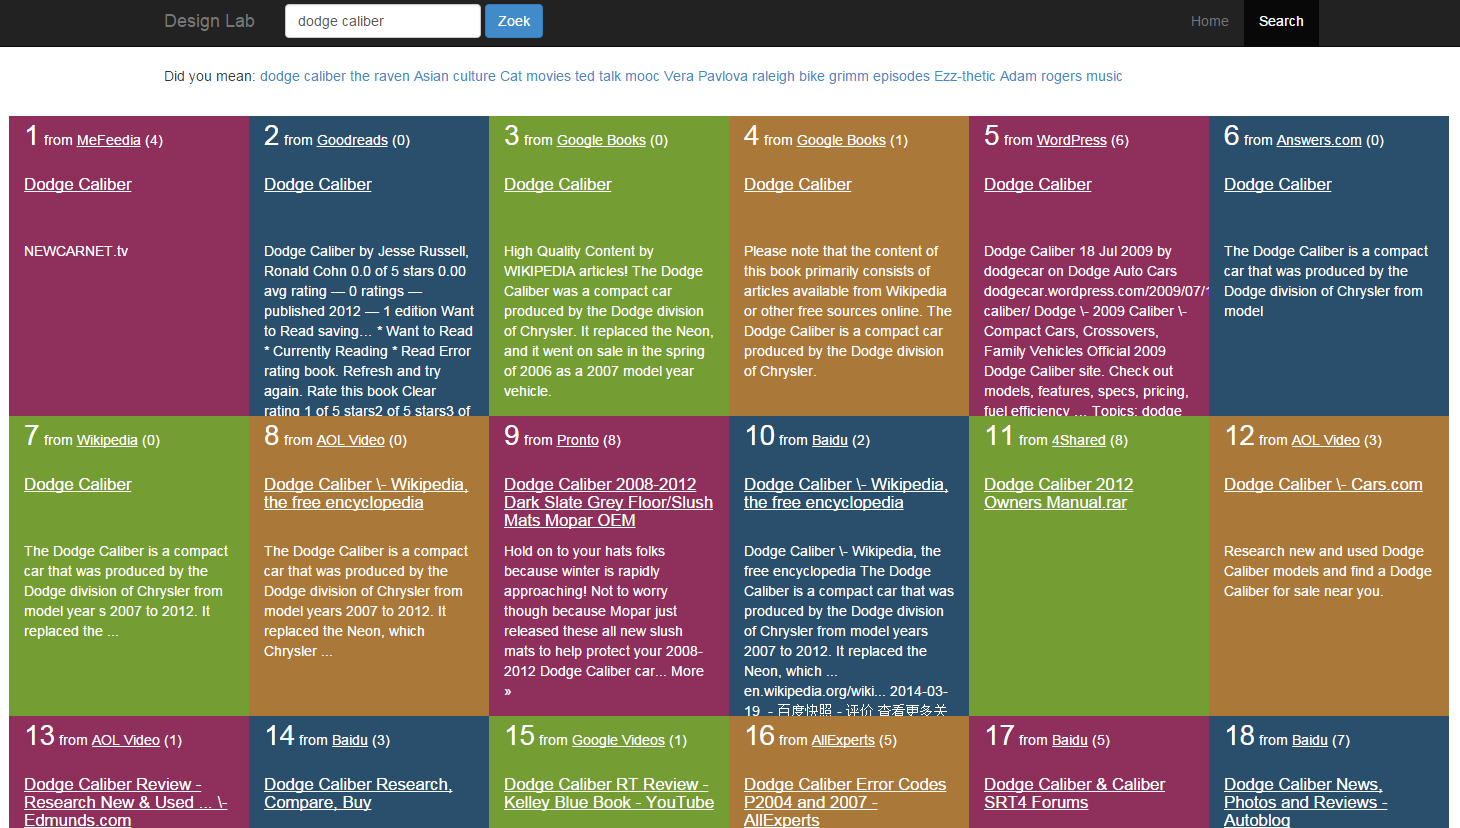
\includegraphics[width=1.0\textwidth]{designOne.png}
  \caption{Screenshot of Design One.}
\label{fig:designOne}
\end{figure}

Each block in the design represents a search result with its title, description, and a link to the original source. 
Each block has the same width and height to give each result the same importance. 
Furthermore the top left result is the first result and can be seen as the most relevant result to the query.
As can be seen from the result reports the relevance is ordered from left to right, and then from top to bottom. 
The source is also shown in the block of each result.
This allows the user to scan the results for results of specific search engines. 

In our design the whole screen is used, such that there is no unused space. 
The blocks will also float to other screen sizes, such that each browser has the same, correct display of the result page.
The dynamic setup of the design allows us to show as much information to the user as possible. 
However, it should be noted that too much information can distract the user, making searching for a desired result inefficient.
By giving each search result the same width and height, and thus a structured result page, we aim to prevent this. 

% Rik's layout
\subsection{Design Two}
\label{sec:layoutRik}
The second design (Design Two, see figure~\ref{fig:designTwo}) has an other approach than our first design.
In this design the results are ordered by category first before ordering by relevance.
In order to do this each search engine had to be allocated to a category.
For this we used the file \textit{FW14-engines.txt}, which consists of all search engines used to generate the FedWeb result data.
In total 21 categories were used to group similar search engines, and thus there search results, together.
In table~\ref{tab:selectionRik} in appendix~\ref{app:enginetypes} the allocation of the search engines to categories is shown.

\begin{figure}[h!]
  \centering
    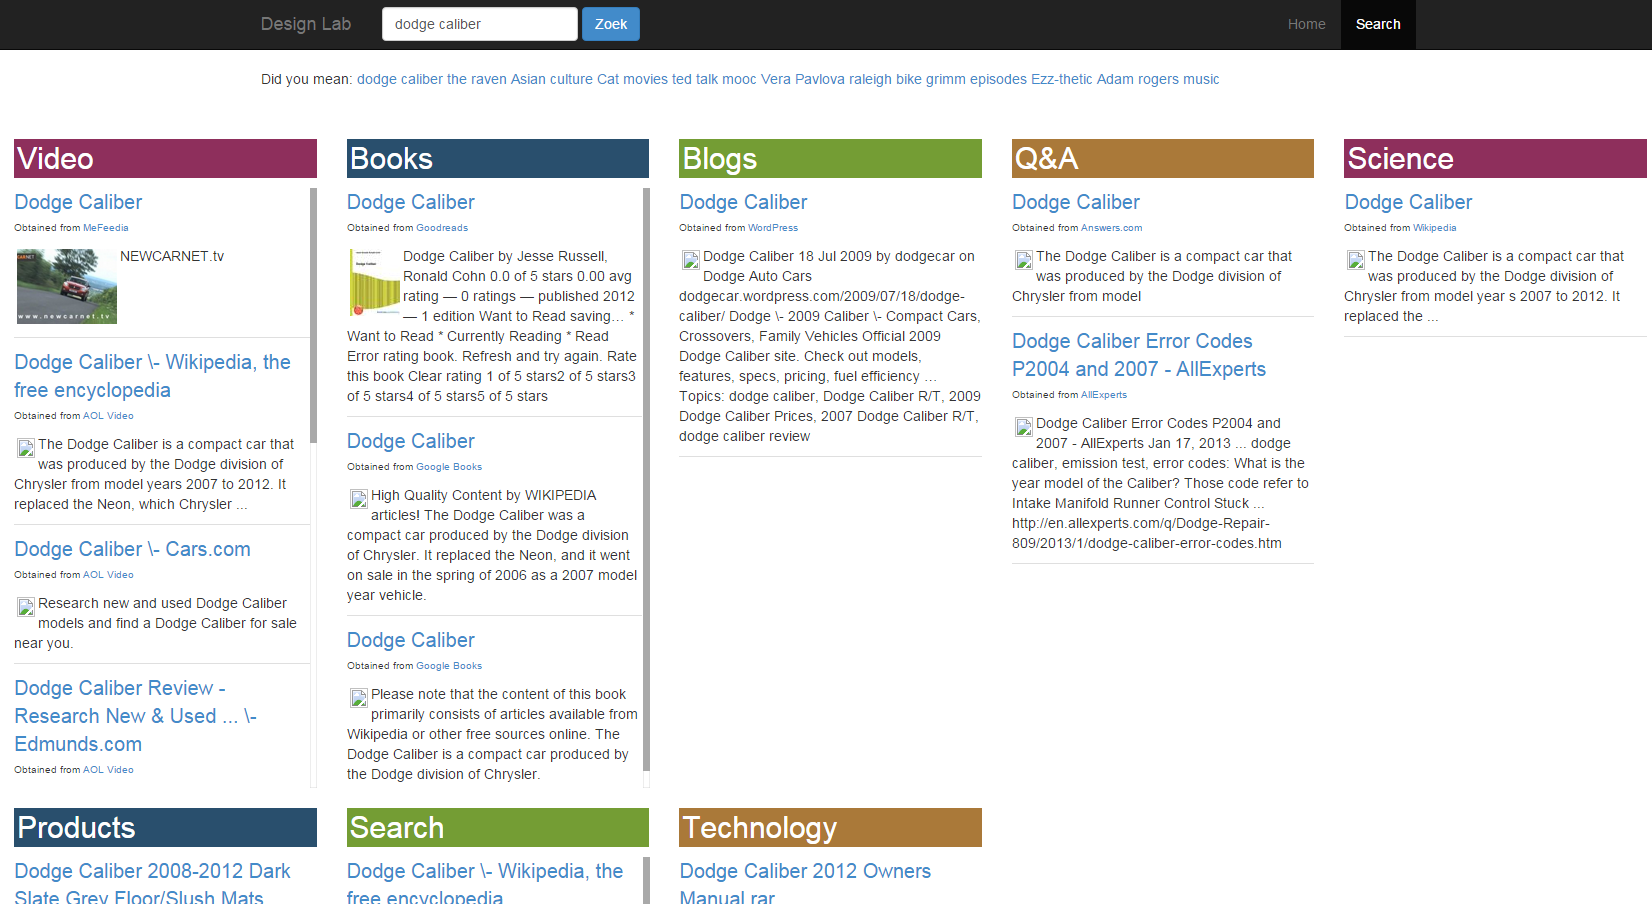
\includegraphics[width=1.0\textwidth]{designTwo.png}
  \caption{Screenshot of Design Two.}
\label{fig:designTwo}
\end{figure}

The design is built while keeping in mind the current use of widescreens.
In our opinion long vertical lists may not be the most userfriendly for widescreens, thus we looked into a design that has a more horizontal approach.

The design consists of an undefined number of rows with each consisting of a maximum of five categories.
The categories are sorted based on the retrieval of the results, so the category of the first retrieval will be the category in the upper left of the display, the next new category will be next to it on the right, et cetera.
Each category takes up 20\% of the total screen width.
This is chosen to maximize the available space on screens instead of waisting space because it is considered more modern.

Each row has a maximum height, such that the user can see already more categories if there are more than five.
It should make the user immediately aware of the fact that there are more types of search results, instead of having to scroll down first.

We decided to not develop a responsive layout due to time constraints.
Therefore it is important to note that this design was developed on a computer system with a screen resolution of 1680 x 1050 pixels.
When using this resolution, or a higher resolution like 1920 x 1080 pixels, the display of the design should be correct.
When considering the screen width, all resolutions from 1024 x 768 pixels and higher should be able to display five categories beside each other, although the text might be not userfriendly to read at the lower resolutions.
When considering the screen height, all resolutions from 1280 x 1024 pixels and higher should be able to display the headings of the second row of categories.

\section{How to evaluate this project designs}
\label{sec:evaluation}
To test our designs we have to establish at least two designs to compare. 
In order to get a good comparison we need to control the variables of the design. 
The user has a question in mind, and which design will answer that question the best. 

To perform this evaluation we need to have a control, which can be in our case the 10 results for each search engine in a tabbed environment. The user can find the information by clicking the right tab and will find the information in that tab. The other designs we have are blended designs.

We will test two things. Are the results the correct results and how fast will the user find his answer. 

To find out if a design performs better than the baseline we will measure the time the user will have its answer. The faster the user finds its answer the better. We will measure this by the time the user enters the query until clicking on the answer page. In order to perform this evaluation several test subjects are needed that will perform several queries on the different designs. They never will have to do the same query in at two designs, because that will give them some notion of what they are looking for. So, every person has to perform 30 queries. 10 on the base design, 10 on version 1 and 10 on version 2. The time is compared for the same query for different persons.

To automate this process our blended designs are evaluated with a list of answers pages the experts described by~\cite{lalmas2011aggregated} have given for each query. Our automated blended design must have those answers as a result, or else our design is wrong. The more results pages we have the experts have given the better our design is performing. This can be automatic by counting the results which are in the result or not. 

When both tests result in that some design is better than the other we will say that the design is better. % wut :P

\section{Conclusions}
\label{sec:conclusion}
We developed two different designs for a web result page.
Design One presents the search results in equally sized blocks, ordered only by relevance.
Design Two on the other hand orders by category first, followed by an order by relevance within each category.
Since both designs are mainly based on their type of ordering, it seems clear that the way of ordering has a large influence on a design.
However, if one or both of our designs are `good' designs cannot be concluded at this moment.
To determine this our designs should be compared to other designs of result pages, for example by an execution of our proposed evaluation.

\section{Checklist}
\begin{enumerate}
\item Check if our readme is valid with a new clean install
\item Rik: reports van mijn layout controleren
\end{enumerate}

\bibliographystyle{abbrv}
\bibliography{libfile}

\appendix
\section{Search Engine Types}
\label{app:enginetypes}
\begin{center}
\begin{table}
  \begin{tabular}{ | l | l | }
    \hline
    \textbf{Type} & \textbf{Search engines} \\ \hline
Blogs
& 	Google Blogs	\\
& 	LinkedIn Blog	\\
& 	Tumblr	\\
& 	WordPress	\\
\hline
Books
& 	Goodreads	\\
& 	Google Books	\\
& 	NCSU Library 	\\
&	Wikibooks	\\
\hline
Career
& 	Glassdoor	\\
& 	Jobsite	\\
& 	LinkedIn Jobs	\\
& 	Simply Hired	\\
& 	USAJobs	\\
\hline
Comedy
& 	Comedy Central Jokes.com	\\
& 	Kickass jokes	\\
\hline
Entertainment
& 	E! Online	\\
& 	Entertainment Weekly	\\
& 	TMZ	\\
\hline
Food
& 	AllRecipes	\\
& 	Cooking.com	\\
& 	Food Network	\\
& 	Food.com	\\
& 	Meals.com	\\
\hline
Games
& 	Addicting games	\\
& 	Amorgames	\\
& 	Crazy monkey games	\\
& 	GameNode	\\
& 	Games.com	\\
& 	Miniclip	\\
\hline
Health
& 	Centers for Disease Control and Prevention	\\
& 	Family Practice notebook	\\
& 	Health Finder	\\
& 	HealthCentral	\\
& 	HealthLine	\\
& 	Healthlinks.net	\\
& 	Mayo Clinic	\\
& 	MedicineNet	\\
& 	MedlinePlus	\\
& 	University of Iowa hospitals and clinics	\\
& 	WebMD	\\
\hline
Images
& 	DeviantArt	\\
& 	Flickr	\\
& 	Fotolia	\\
& 	Getty Images	\\
& 	IconFinder	\\
& 	NYPL Gallery	\\
& 	OpenClipArt	\\
& 	Photobucket	\\
& 	Picasa	\\
& 	Picsearch	\\
& 	Wikimedia	\\
& 	Funny or Die	\\
\hline
Kids
& 	Cartoon Network	\\
& 	Disney Family	\\
& 	Factmonster	\\
& 	Kidrex	\\
& 	KidsClicks!	\\
& 	Nick jr	\\
& 	OER Commons	\\
& 	Quintura Kids	\\
\hline
Music
& 	LastFM	\\
& 	LYRICSnMUSIC	\\
\hline
News
& 	BBC	\\
& 	Chronicling America	\\
& 	CNN	\\
& 	Forbes	\\
& 	JSOnline	\\
& 	Slate	\\
& 	The Street	\\
& 	Washington post	\\
\hline
Products
& 	Amazon	\\
& 	ASOS	\\
& 	Craigslist	\\
& 	eBay	\\
& 	Overstock	\\
& 	Powell's	\\
& 	Pronto	\\
& 	Target	\\
& 	Yahoo! Shopping	\\
\hline
Q\&A
& 	AllExperts	\\
& 	Answers.com	\\
& 	Chacha	\\
& 	StackOverflow	\\
& 	Yahoo Answers	\\
& 	MetaOptimize	\\
& 	HowStuffWorks	\\
\hline
Science \& Knowledge
& 	arXiv.org	\\
& 	CCSB	\\
& 	CERN Documents	\\
& 	CiteSeerX	\\
& 	CiteULike	\\
& 	eScholarship	\\
& 	KFUPM ePrints	\\
& 	MPRA	\\
& 	MS Academic	\\
& 	Nature	\\
& 	Organic Eprints	\\
& 	SpringerLink	\\
& 	U. Twente	\\
& 	UAB Digital	\\
& 	UQ eSpace	\\
& 	PubMed	\\
& 	Wikipedia	\\
& 	Wikispecies	\\
& 	Wiktionary	\\
& 	National geographic	\\
\hline
Search
& 	About.com	\\
& 	Ask	\\
& 	CMU ClueWeb	\\
& 	Gigablast	\\
& 	Baidu	\\
\hline
Social
& 	Foursquare	\\
& 	Myspace	\\
& 	Reddit	\\
& 	Tweepz	\\
\hline
Sport
& 	bleacher report	\\
& 	ESPN	\\
& 	Fox Sports	\\
& 	NHL	\\
& 	SB nation	\\
& 	Sporting news	\\
& 	WWE	\\
\hline
Technology
& 	HNSearch	\\
& 	Slashdot	\\
& 	The Register	\\
& 	4Shared	\\
& 	Cnet	\\
& 	GitHub	\\
& 	SourceForge	\\
& 	Ars Technica	\\
& 	CNET	\\
& 	Technet	\\
& 	Technorati	\\
& 	TechRepublic	\\
\hline
Travel
& 	TripAdvisor	\\
& 	Wiki Travel	\\
\hline
Video
& 	Comedy Central	\\
& 	Dailymotion	\\
& 	YouTube	\\
& 	IMDb	\\
& 	5min.com	\\
& 	AOL Video	\\
& 	Google Videos	\\
& 	MeFeedia	\\
& 	Metacafe	\\
& 	Veoh	\\
& 	Vimeo	\\
& 	Yahoo Screen	\\
& 	BigWeb	\\
\hline
  \end{tabular}

\caption{Types of search engines}
\label{tab:selectionRik}

\end{table}
\end{center}

\end{document}
